\chapter{Theory}
\label{chap:theory}

\initial{T}his thesis is comprised of experimental searches for dark matter and new physics. The experimental chapters Chpt.~\ref{chap:higgstoinv} and Chpt.~\ref{chap:svj} delve deeply into the analyses. Before which, the theoretical and phenomenological motivations must be understood to [back up] the need for these searches at the \acrlong{lhc}. In this chapter, a brief recap of the \acrlong{sm} will be [presented] along with its shortcomings, i.e., the lack of a dark matter candidate. Theoretical descriptions of dark matter that best fit the relic density and astrophysical observations will then be discussed. Specific interpretations in the form of \glspl{svj} and invisibly decaying Higgs bosons are [looked at] that provide the background for the respective analysis chapters.


%=========================================================


\section{The standard model of particle physics}
\label{sec:standardmodel}

\begin{easylist}[itemize]
    \easylistprops
    & Give an overview of the fundamental forces and particles.
    & Discuss the Standard Model in some amount of detail, emphasizing certain aspects as they relate to the Higgs field (and boson).
    & May have to mention chirality and helicity in relation to "handedness" of particles
    & Mention resonances and widths. Each decay mode of a particle contributes a partial width (which determines its branching ratio - BR = partial width/total width)
    & Talk in some detail about the Higgs mechanism as that will inform the Higgs to invisible section. Mention Yukawa coupling to fermions, and that it's dependent on the squared mass of the decay products. Lends credence to suppression of direct decay to neutrinos (assuming they even couple to Higgs)
\end{easylist}

% Check Lancaster and other summer school notes (Postgraduate and CMS courses/ folder)



%=========================================================


\subsection{Limitations of the standard model}
\label{subsec:sm_limitations}

% Check Lancaster and other summer school notes for other limitations, specifically referencing things that can tie into dark matter

Despite the \acrlong{sm} providing precise predictions of three of the four fundamental forces and the particles that they interact with, there are many experimental observations that it cannot currently explain. Neutrino masses, dark matter, dark energy, and gravity all escape its description.

The hierarchy problem is one of the more serious issues facing the \acrlong{sm}. It may be explained in different manners that emphasize a certain aspect. Fundamentally, it is a question of the disparity between energy scales of the fundamental forces (particularly relating to the weak scale and gravity). The masses of the intermediate vector, and Higgs, bosons \OrderOf{\text{100\GeV}/c^2} are much smaller than than the Planck mass \OrderOf{\text{10}^{19}\GeV/c^2}. The mass term for the Higgs boson is $m^2 H^{\dagger} H$ in the \acrshort{sm}. Invariance under a gauge or global symmetry in the Higgs field $H$ leads to the mass being open to radiative corrections all the way up to the Plank scale.\footnote{Justify this more?} It appears that, in nature, these very large terms cancel to [give] the familiar $m_{\PH} = \text{125}\GeV/c^2$~\cite{Chatrchyan:2012xdj,Aad:2012tfa}. It is deemed unnatural to expect a cancellation to such a degree, i.e., one part in 10$^{17}$. This \emph{fine-tuning} of parameters in the \acrlong{sm} is something that unified or natural theories desperately try to avoid.

Some \acrshort{bsm} theories like \acrlong{susy} provide well-motivated cancellations by introducing supersymmetric particles. In certain implementations, some of these supersymmetric particles should exist at the \tTeV energy scale. In the \acrshort{sm}, the largest correction to the Higgs mass derives from the top quark, since its Yukawa coupling to the Higgs is the strongest. At one-loop order, new physics at \OrderOf{\tTeV} scale is required, with new particles coupling to the Higgs field to prevent these corrections from being unreasonably large~\cite{Farina:2013ssa}. Arguments such as this give credence to new physics being discoverable at particle accelerators such as the \acrlong{lhc}.


%=========================================================


\section{Theoretical motivations for, and descriptions of, dark matter}
\label{sec:theory_dark_matter}

% Will probably be referring to things from introduction section. Try to just give overview there and describe the nitty-gritty here

The universe may have conjured dark matter via one of many possible mechanisms. The most popular is described as a ``thermal freeze-out'' process. In the hot, early universe when the thermal background allowed spontaneous pair production of particle dark matter, it was produced in abundance. During this period, the particles may also have frequently annihilated since the cosmos was still small. Inevitably, the universe expanded and cooled; the temperature became too low to allow significant production \cite{Baldes:2017gzw}. Matter was further separated and the dark matter annihilation rate decreased, leaving a behind the ``thermal relic'' that is observed today. These remaining particles were attracted via gravity, forming filaments throughout the universe. The potential wells they induced allowed the progenitors of galaxies to form within.

Full derivations of the thermal freeze-out of dark matter\footnote{Is it worth going through the derivation, maybe as an appendix? It might be superfluous considering it's already described in literature.} can be found in literature \cite{cosmic_abundances_stable_particles,Bender:2012gc}, with the ``\acrshort{wimp} miracle'' as a consequence: with relatively few assumptions, the correct dark matter relic abundance can be recovered by requiring a \acrshort{wimp} mass of \OrderOf{\text{\tGeV} - \text{\tTeV}}, dependent on the annihilation cross section. This is a range accessible at contemporary colliders such as the \acrshort{lhc}, and perhaps coincidentally, around the electroweak energy scale. It is common for figures that depict the \acrshort{wimp} dark matter density over time to plot the ``yield'' $\sfrac{n_{\chi}}{s}$ as a function of the dimensionless parameter $x = \sfrac{m_{\chi}}{T}$. In the former variable, $n_{\chi}$ is the number density and $s$ is the entropy density. In the latter, $m_{\chi}$ is the dark matter mass and $T$ is the average temperature of the universe, which serves as a measure of its age since the temperature decreases over time. An example is given in Fig.~\ref{fig:theory_dm_abundance}.

\begin{figure}[htbp]
    \centering
    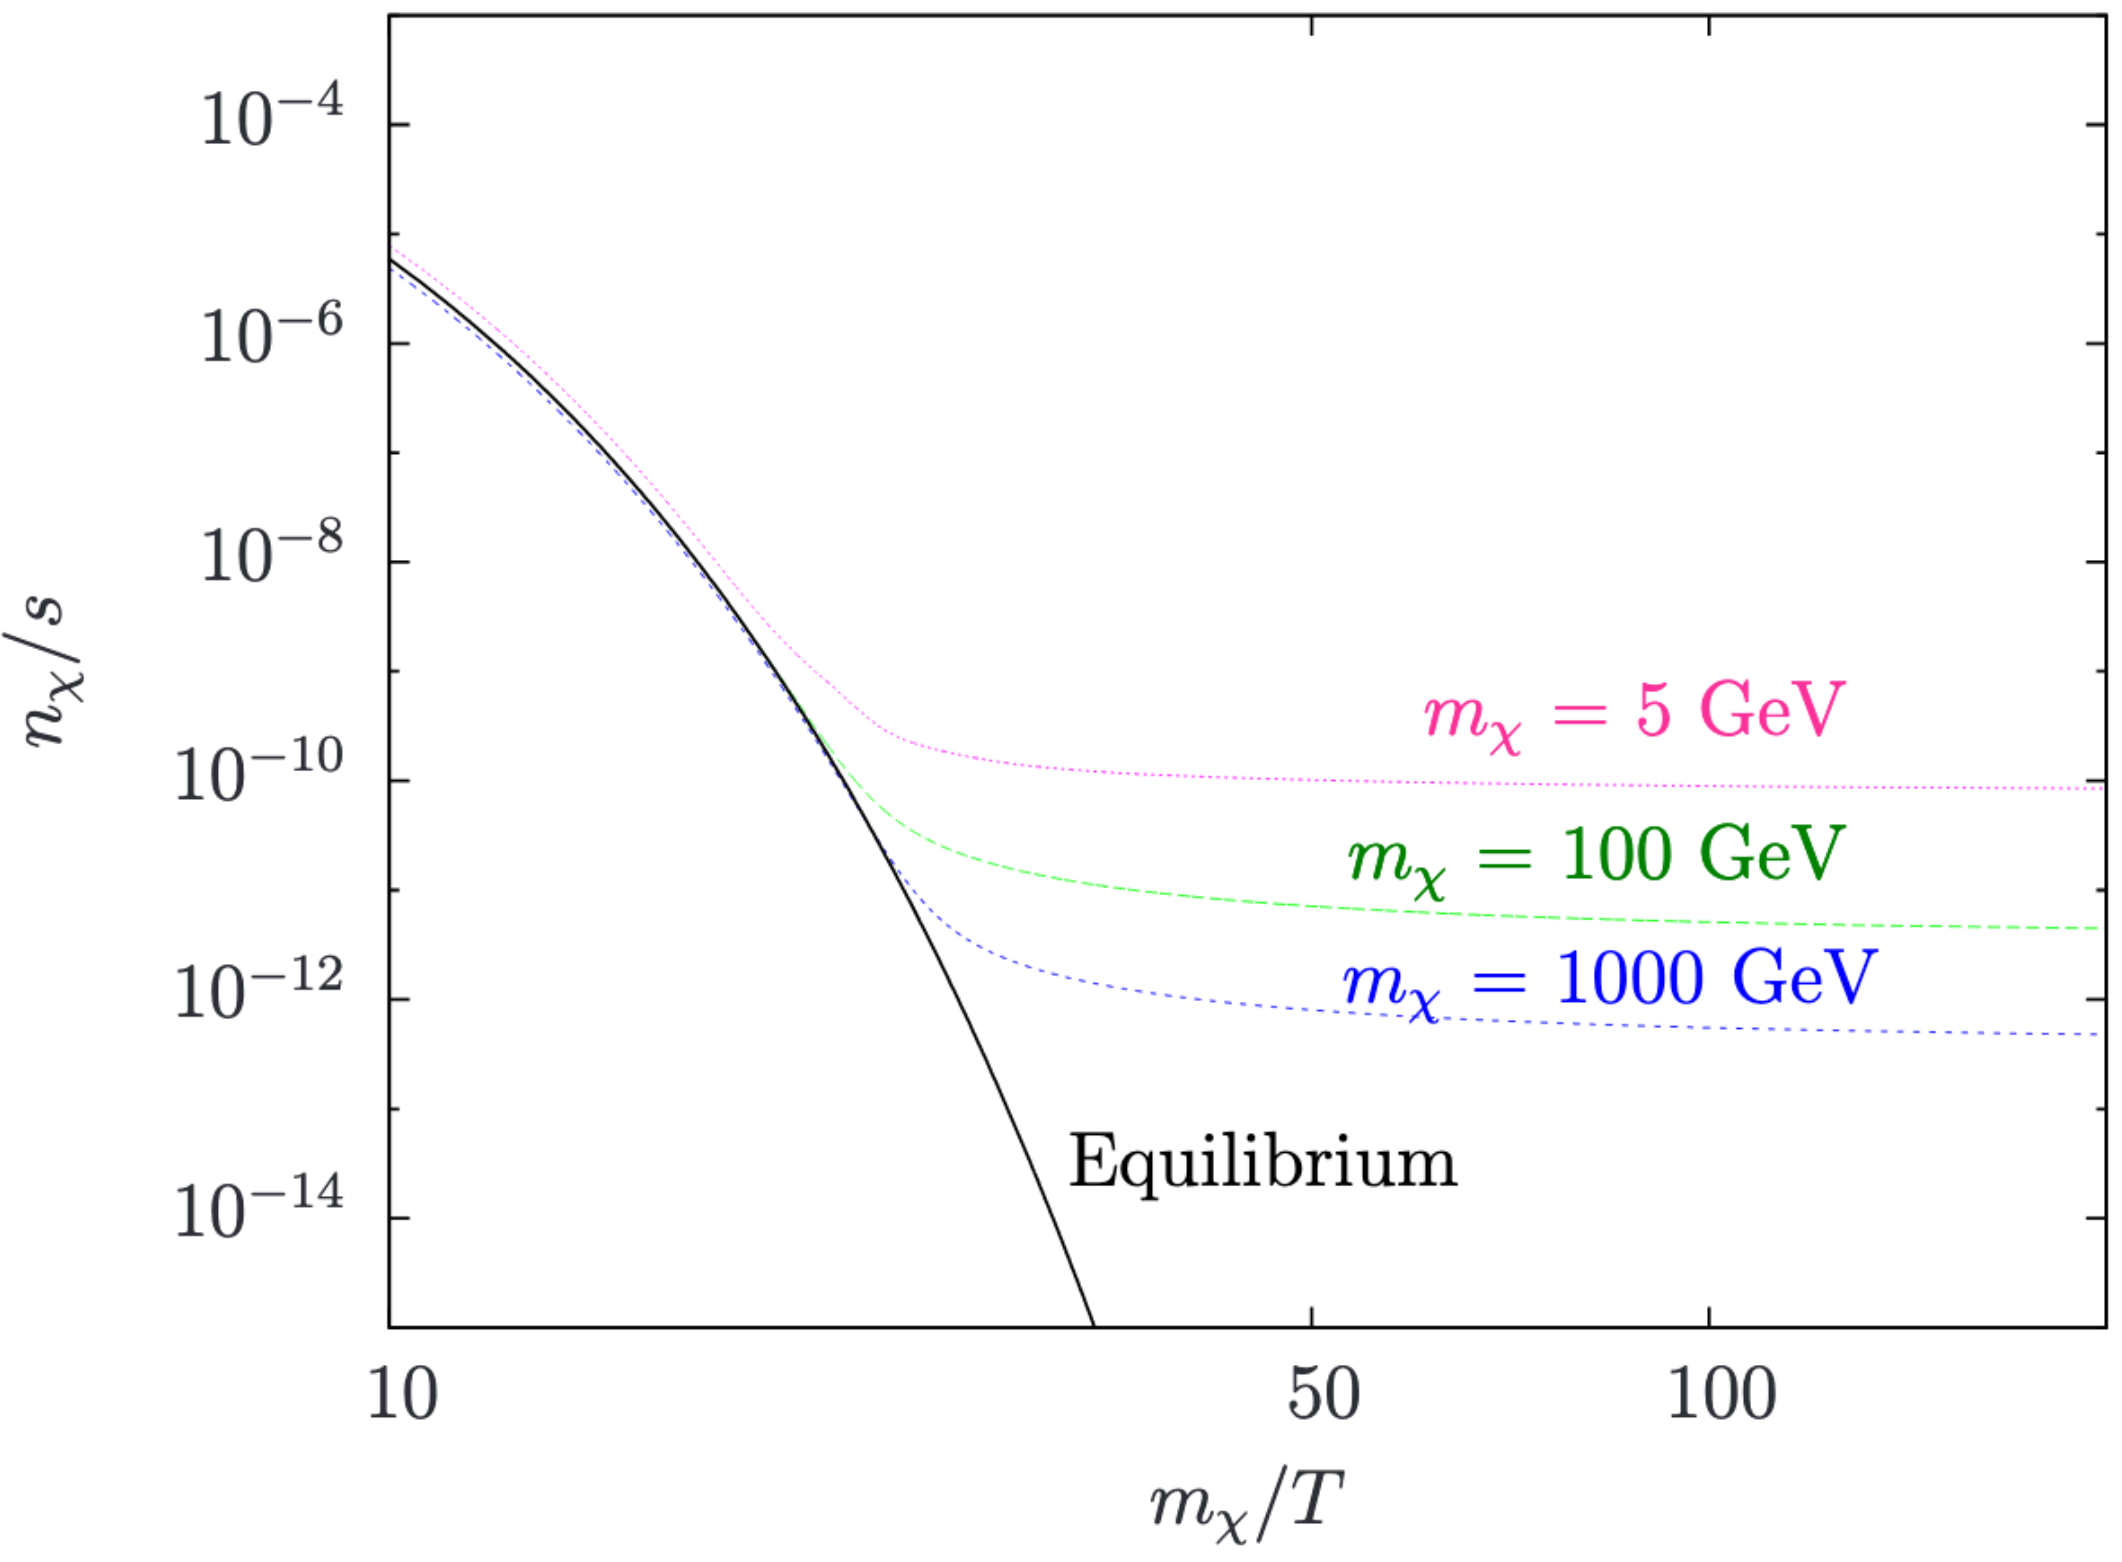
\includegraphics[width=0.75\textwidth]{figures/dm_abundance.png}
    \caption[A measure of \acrshort{wimp} dark matter comoving number density as a function of time with projections for different particle masses]{A measure of \acrshort{wimp} dark matter comoving number density as a function of time with projections for different particle masses. A higher mass must be balanced by a larger annihilation cross section to achieve the correct relic density, to which it tends asymptotically from the point of thermal freeze out. The black curve represents the scenario in which dark matter remains in equilibrium with the \acrlong{sm}. Figure taken from Ref.~\citenum{Han:2013gba}.}
    \label{fig:theory_dm_abundance}
\end{figure}

The time of the dark matter freeze out epoch is somewhat insensitive to the mass and annihilation cross section. Approximate solutions to the Boltzmann equation for time-dependent $n_{\chi}$ --- where dark matter is modelled as a weakly-interacting, diffuse gas of particles --- suggest $x_f \sim 20$~\cite{Lisanti:2016jxe,Bender:2012gc}. Stronger dark matter interaction leads to decoupling at a later time and a lower number density. The approximate value of $x_f$ is significant in that it supports the electroweak-scale mass of \glspl{wimp}.

Another popular mechanism, targeting low-mass dark matter, is the ``freeze-in'' process~\cite{Hall:2009bx,Krnjaic:2017tio}. In this [scenario], dark matter is not produced thermally in the early universe. Instead, it emerges through interactions between \acrshort{sm} particles such as collisions, or decays of those heavier than dark matter. The comoving density increases with time until it plateaus because of the cooling of the universe, where \acrshort{sm} particles are generally stable enough and too low energy to produce dark matter in any meaningful quantity. The relic abundance can therefore reclaimed from a combination of the initial thermal distributions, the dark matter mass, and the interaction strength, similar to the freeze-out process. In order to obey cosmological observations, particularly the fact that it is cold, the masses freeze-out dark matter particles are expected to be \OrderOf{\text{k\acrshort{ev}}} or heavier.

% Could also briefly describe other interpretations of dark matter relic abundance. For all of these cases, perhaps I can explain them more qualitatively with no/few equations (but reference derivations in literature), and add footnotes questioning how much detail I _should_ go in to.

% DON'T RENDER
\iffalse

% Taken directly from my lab book. Tidy up and improve
\begin{easylist}[itemize]
\easylistprops
& The mediator (force-carrying particle, like the gauge bosons) for dark matter -- between dark matter particles or the dark matter-Standard Model particle interactions -- may be a scalar (spin-0, like the Higgs boson) or pseudoscalar (reverses parity under a Lorentz transformation, like the pion) boson. [Support] for a pseudoscalar over a scalar mediator comes from the Feynman diagrams for DM annihilation into, e.g., \Pqb-quarks. With a scalar mediator, the vertex factors and the propagator term lead to cancellations in the cross section equation in the low-velocity limit.

& The mediator for dark matter may be heavier than the dark matter particle itself (like with the $W^{\pm}$ and \PZ bosons being heavier than most of the particles they mediate), maybe 2x heavier or more so than the DM particle. The mediator could decay via DM pair production, so it makes sense that it would be at least twice as heavy.

& There's no consensus on whether dark matter is fermionic or bosonic. If fermionic, it may be either a Dirac fermion (particle is distinct from its antiparticle, like the electron and positron) or Majorana fermion (particle is the same as its antiparticle, like the neutrino is \underline{suspected} to be). If it were Majorana, dark matter could annihilate with itself, making discoveries via indirect searches more likely.

& Some good results showcasing dark matter masses and that of its mediator from different analyses and decay channels are at \cite{CMS-DP-2016-057}. Particularly figures 4 and 6, which I used in my poster for the PGR conference.

\end{easylist}


% Taken directly from my lab book. Tidy up and improve. Look through these papers to see which ones give compelling interpretations and motivation for dark matter
Papers to look at regarding SUSY and dark matter:

\begin{easylist}[itemize]
\easylistprops
& \cite{dmsearcheslhc2015}
& \cite{dmbenchmarkearlylhcrun2}
& \cite{CMS-PAS-EXO-12-055}
& \cite{Aitchison:2005cf}
& \cite{Ellis:2002mx}
& \cite{Murayama:2007ek}
& \cite{Peskin:2007nk}
& \cite{Goodman:2010ku}
& \cite{PhysRevLett.115.181802}
& \cite{CMS:2016pod}
& \cite{Bertone:2004pz}
\end{easylist}

\fi


%=========================================================


\section{Important observables and quantities in collider physics}
\label{sec:theory_important_observables}

The following section discusses some ubiquitous variables and units in high energy physics, particularly in the context of colliders. Subsequently, it is [useful] to consolidate their definitions here.\footnote{The theory chapter is probably not the right place to put this section. Maybe a separate section or appendix would be better.}


%=========================================================


\subsection{The electron volt}
\label{subsec:theory_electron_volt}

In highly relativistic systems, such as beams of particles in accelerators, the ability to simply equate mass, energy, and momentum is desirable. In the \acrshort{lhc}, when protons are accelerated to an enormous Lorentz boost factor, their invariant mass $m_0$ contributes little to their total energy $E$. With Einstein's energy-momentum relation from special relativity, one can express mass and momentum in units of energy:

\begin{equation}
    E = \sqrt{ (pc)^2 + (m_0c^2)^2 }
    \label{eq:theory_e_mc2}
\end{equation}

where $p$ is the magnitude of the momentum and $c$ is the speed of light. For highly relativistic objects, $pc \gg m_0c^2$ and so $E \approx pc$. At rest, $E = m_0c^2$. The \acrfull{ev} unit is common in high energy physics. Its value is the energy supplied to (or removed from) an electron accelerated through a potential difference of 1\,V, i.e., $\text{1.6}\times \text{10}^{-19}$\,J. The momentum gained is then $\text{1\,\eV}/c$ and relativistic mass $\text{1\,\eV}/c^2$. The factors of $c$ and $c^2$ are often dropped in less formal contexts, or when using natural units (where $c = \text{1}$).

An electron volt is a minute quantity of energy, so when discussing properties of high energy particles and accelerators, a long string of digits may be required to express them. SI prefixes mitigate this problem and provide an intuitive sense of scale to scientists. The most frequently used in the context of \acrshort{lhc} physics are \emph{mega} (M, $\text{10}^6$), \emph{giga} (G, $\text{10}^9$), and \emph{tera} (T, $\text{10}^{12}$). For example, the mass of a proton is $\text{0.93}\GeV/c^2$ and the present centre of mass energy of the \acrshort{lhc} is $\text{13}\TeV$, which are much more natural and understandable numbers than $\text{1.78}\times \text{10}^{-27}$\,kg or $\text{1.6}\times \text{10}^{-7}$\,J, respectively.


%=========================================================


\subsection{Transverse momentum (\texorpdfstring{\pt}{pt})}
\label{subsec:theory_pt}

In the LHC (or any other collider), the longitudinal momentum of the initial state particles is typically unknown. However, the momentum transverse to the beam is zero before the collision, and therefore must be zero afterward after due to momentum conservation. This is why the transverse momentum of a particle or physics object (\ptvec for the vector quantity, \pt for its magnitude) is a useful variable in an analysis.

% Do I need a more formal/mathematical definition, or a diagram?


%=========================================================


\subsection{\texorpdfstring{\HT}{HT}}
\label{subsec:theory_ht}

% Will need to define what a jet is here if I don't do so before

The scalar sum of the transverse momentum of hadronic constituents in an event, i.e., the \glspl{jet}, is symbolised as \HT. It is often used in analyses focused on hadronic objects, such as natural \acrlong{susy} in which a large jet multiplicity is expected. Formally,

\begin{equation}
    \HT \equiv \sum_{\mathrm{jets}} \pt
    \label{eq:ht_definition}
\end{equation}

Typically, a lower limit on \pt is used when calculating the \HT, so jets below this threshold do not factor into the sum. This is to avoid low momentum jets attributed to pileup events (see Chpt.~\ref{subsec:pileup}), and those from the primary vertex that can often be mismeasured.


%=========================================================


\subsection{Missing transverse momentum (\texorpdfstring{\ptmiss}{ptmiss})}
\label{subsec:theory_met}

The missing transverse momentum \ptmiss is defined as the negative vector sum of the \pt of all identified particles in an event. It is a term often used interchangeably with \gls{met} (MET, \glssymbol{met}). Undetected particles from neutrinos or dark matter, or mismeasured kinematic properties of identified particles, will introduce an imbalance in the vector sum of the \pt. Hence, the \ptmiss will be non-zero. Formally,

\begin{equation}
    \ptmiss \equiv - \sum_i^{N_{\mathrm{particles}}} \vec{p}_{\mathrm{T}, \, i}
    \label{eq:met_definition}
\end{equation}

The hadronic-only counterpart to this variable, \mht, is the negative vector sum of the jet transverse momenta in an event:

\begin{equation}
    \mht \equiv - \sum_j^{N_{\mathrm{jets}}} \vec{p}_{\mathrm{T}, \, j}
    \label{eq:mht_definition}
\end{equation}

As with \HT, the \mht is often calculated with a lower limit on the jet \pt.

% A depiction of the MET (e.g., SM particles recoiling off dark matter) might be useful for the reader


%=========================================================


\section{Measuring the branching ratio of invisibly decaying Higgs bosons}
\label{sec:theory_higgs_to_inv}

The Higgs boson has caught the attention of the high energy physics community and even the public eye like no other particle in recent memory. Its discovery in the $\HepProcess{\PH \to \Pphoton\Pphoton}$ channel in 2012 by both \acrshort{cms}~\cite{Chatrchyan:2012xdj} and \acrshort{atlas}~\cite{Aad:2012tfa} independently realised one of the [principal] goals of the LHC's construction. The particle itself is not necessarily exciting. Rather, it confirms the existence of the Higgs \emph{field} that pervades the universe and gives mass to the elementary particles via the exchange of its namesake boson~\cite{PhysRevLett.13.321,PhysRevLett.13.508,PhysRevLett.13.585}. [Its discovery], one might think, was the end of the discussion of the Higgs boson. However, it was only the beginning.

Many observations of the Higgs, such as its predominant decay mode $\HepProcess{\PH \to \Pqb\APqb}$, were not seen until recently (\acrshort{cms}~\cite{Sirunyan:2018kst}, \acrshort{atlas}~\cite{Aaboud:2018zhk}). Constraints on its other properties have also been placed, such as its resonance width and branching ratios \BR to other final states. Fully understanding the Higgs boson is important to understanding the Higgs field and the wider \acrlong{sm}. Precision measurements in tension with \acrshort{sm} predictions can also be a window to new physics. Measuring the \higgstoinv branching ratio aims to do just that.

The only \acrshort{sm} process in which Higgs boson can decay invisibly\footnote{A direct decay to neutrinos is possible if they acquire their mass from the Higgs field. But as the coupling is of a Yukawa form and the upper limit on the \acrshort{sm} neutrino masses is very small, the branching ratio is expected to be heavily suppressed.} is $\HepProcess{\PH \to \PZ\PZ \to 4\nu}$ with a branching ratio of \OrderOf{\text{0.1\,\%}}~\cite{Heinemeyer:1559921}. The leading observed experimental upper limits on this measurement are 19\,\% from CMS~\cite{Sirunyan:2018owy} and 26\,\% from \acrshort{atlas}~\cite{Aaboud:2019rtt}, far above the predicted value. If undiscovered invisible particles, perhaps dark matter, couple to the Higgs field the branching ratio will be enhanced.\footnote{Do I need to give a more mathematical motivation for the BR being enhanced/what kind of values the BR is expected to be from various DM models?} Experimental evidence shows the coupling strength to proportionally follow the mass of the particle, as verified in \acrshort{atlas} and \acrshort{cms}' latest measurements~\cite{Sopczak:2708121}. A considerably large enhancement may allow for this process to be observed at the \acrshort{lhc}. At the very least, a more accurate constraint on the branching ratio is able to exclude some models of dark matter, such as those described in Refs.~\citenum{Djouadi:2012zc,KAKIZAKI201544}.

There is no reason to assume dark matter does \emph{not} interact with the Higgs field, since it bestows mass to all known elementary particles (a small caveat, perhaps, being neutrinos).\footnote{Do I need to give some mathematical motivation as to \emph{why} dark matter would couple to the Higgs? Or is the fact that it has mass enough justification?} Higgs ``portal'' models have been theorised that connect the visible sector of the \acrlong{sm} to a dark sector where particle dark matter resides~\cite{higgs_portal_singlet_dm,Arcadi:2019lka}. Certain models also predict a detectable presence at the \acrshort{lhc} from a sufficient production rate~\cite{Boveia:2018yeb}, perhaps even with data obtained during Run-2~\cite{Abercrombie:2015wmb}.

% If models exist, mention briefly about potential theories with dark matter candidates being able to fix the hierarchy problem (present in a mathematical context if possible).


%=========================================================


\section{Searches for semi-visible jets}
\label{sec:theory_svj}

Many searches for dark matter presume it is a \acrshort{wimp}-like particle because of the considerations discussed in Chpt.~\ref{sec:theory_dark_matter}. In the \acrshort{lhc}, the signatures of \glspl{wimp} would be driven by large missing transverse momentum recoiling from visible matter in the event. Monojet~\cite{Khachatryan:2014rra} and dijet~\cite{Sirunyan:2016iap} searches are able to exploit this, for example. However, no sign of \glspl{wimp} have been observed yet. Thankfully, a boundless supply of [other] theories exist, with possible signatures equally as varied. Though the \ptmiss could still be one of the characteristics by which the dark matter can be inferred, a plethora of topologies and discriminating observables are possible. The dynamics that govern dark matter may be confined to a ``dark sector'' or ``hidden sector'', inhabited by new forces and particles.

A dark sector may be largely inaccessible (as in some Hidden Valley\footnote{A Hidden Valley is a schema where the \acrlong{sm} is extended by a non-abelian group. \acrshort{sm} particles are uncharged under this group. The new, light particles from this extension are the opposite: charged under the new group and neutral under the \acrshort{sm} gauge group. A heavy mediator carries both charges, acting as a portal between the \acrlong{sm} and Hidden Valley particles.} scenarios~\cite{Strassler:2006im}), but communicate with the visible sector through a portal interaction. An example from \acrshort{sm} particles could be the Higgs boson bridging the visible and hidden sectors, as mentioned in Chpt.~\ref{sec:theory_higgs_to_inv}. Many interesting and novel signatures can be probed in \acrshort{lhc} experiments from models like these. Dark forces with energy scales in the tens of \tGeV (gigaelectron volts) and mediator masses up to \tTeV (teraelectron volts) may be accessible. If they are analogous with the \acrlong{sm}, the mechanisms can be explained for the dark matter presence and relic density arising from a baryon-like asymmetry.

Proposed in Refs.~\citenum{Cohen:2015toa,Cohen:2017pzm}, a strongly-coupled dark sector in a Hidden Valley scenario is imagined with interactions analogous to \acrshort{qcd}.\footnote{Do I need to mention that this dark sector is $SU(2)_{\mathrm{dark}}$, and write the lagrangian for how it couples to \acrshort{sm} via dark weak force?} The portals allowing the dark and visible sectors to communicate can be decomposed into a leptophobic \PZprime (\schannel) and bi-fundamental $\Phi$ (\tchannel) mediator. In the \tchannel case, $\Phi$ is a representation of both the visible and dark \acrshort{qcd} gauge groups. Depictions of the processes above are given in Fig.~\ref{fig:theory_svj_portals}. In the \acrshort{lhc}, protons could collide at energies high enough to access the dark sector. From either the resonant production of a \PZprime or exchange of a $\Phi$, dark quarks \Pqdark are produced. Below a dark confinement scale \lamDark, hadronisation takes place into dark hadrons. Depending on the species, some of these dark hadrons are stable (i.e., a source of dark matter), while others are unstable and decay back into visible sector particles, namely \acrlong{sm} quarks. The final state is then a shower of two \glspl{jet} each interspersed with dark matter: \emph{\glspl{svj}}.

\begin{figure}[htbp]
    \centering
    \begin{subfigure}[c]{0.45\textwidth}
    \centering
        \includegraphics[width=0.7\textwidth]{figures/svj/portals_s.pdf}
        \caption{\schannel}
    \end{subfigure}
    \hfill
    \begin{subfigure}[c]{0.45\textwidth}
    \centering
        \includegraphics[width=0.7\textwidth]{figures/svj/portals_t.pdf}
        \caption{\tchannel}
    \end{subfigure}
\caption[Example Feynman diagrams for the two main production modes of semi-visible jets. A \PZprime boson mediates the \schannel process while a bi-fundamental $\Phi$ mediates the \tchannel process]{Example Feynman diagrams for the two main production modes of semi-visible jets \cite{Cohen:2017pzm}. A \PZprime boson mediates the \schannel process while a bi-fundamental $\Phi$ mediates the \tchannel process.}
\label{fig:theory_svj_portals}
\end{figure}


%=========================================================


\subsection{Kinematics and free parameters of the model}
\label{subsec:theory_svj_free_params}

The kinematics of \glspl{svj} are heavily influenced by the [main] free parameters of the model: the mass of the mediator (\mZprime or $m_{\Phi}$), the dark coupling strength (\aDark), the dark quark mass (\mqdark), and the invisible fraction (\rinv).

\begin{easylist}[itemize]
    \easylistprops
    & \mZprime/$m_{\Phi}$: Since the energies of the colliding protons have an upper limit, the conservation of energy (or momentum) imposes one on the on-shell production/exchange of the mediator particle. In the \schannel process, the \PZprime production is resonant. Consequently, its mass is possible to recover by calculating the dijet mass \mjj or transverse mass \mT.

    & \aDark: In Ref.~\citenum{Cohen:2017pzm}, this is defined as $g_{\mathrm{dark}}^2/ 4\pi$ (where $g_{\mathrm{dark}}$ is the coupling constant between the dark quarks and mediator). As in \acrshort{qcd}, the dark coupling runs as a function of the energy scale, influencing \lamDark. At 1\TeV,

    \begin{equation}
        \lamDark = 1000 \ [\mathrm{GeV}] \exp \left( \frac{-2\pi}{\aDark b} \right)
        \label{eq:lambda_dark}
    \end{equation}

    where $b = \frac{11}{3}\Nc - \frac{2}{3}\Nf$ is related to the number of dark colours and flavours, respectively.

    & \mqdark: This parameter does not directly affect much, but is related to the dark hadron mass (2\mqdark) and \lamDark. The combination of the two properties affects the shower dynamics. Note that while Ref.~\citenum{Cohen:2017pzm} describes some of these to be insensitive, a parameter scan over these two variables are necessary in the search described in Chpt.~\ref{chap:svj}.

    & \rinv: This is defined as the fraction of produced invisible particles that remain stable, at least over timescales where they interact with a detector. When generating simulated samples, \rinv can be interpreted as the \emph{probability} of a dark hadron remaining stable. While this variable is not inherent within the model, it is one that can encompass many underlying components. As a result, visualisation of the shower and direction of \ptmiss is much more intuitive, as demonstrated in Figs.~\ref{fig:theory_svj_rinv} and~\ref{fig:theory_svj_met_dir}, respectively. A large value of \rinv would yield a similar final state to a \acrshort{wimp} search.
\end{easylist}

\begin{figure}[htbp]
    \centering
    \includegraphics[width=0.75\textwidth]{figures/svj/r_inv.pdf}
    \caption[The constituents of a semi-visible jet as a function of its invisible fraction]{The constituents of a semi-visible jet as a function of its invisible fraction \rinv \cite{Cohen:2017pzm}.}
    \label{fig:theory_svj_rinv}
\end{figure}
    
\begin{figure}[htbp]
    \centering
    \includegraphics[width=0.85\textwidth]{figures/svj/metfigure.pdf}
    \caption[The typical direction of the missing transverse energy relative to the semi-visible jets as a function of the invisible fraction \rinv]{The typical direction of the missing transverse energy \ETslash\xspace (or \ptmiss) relative to the semi-visible jets as a function of their invisible fraction \rinv \cite{Cohen:2017pzm}.}
    \label{fig:theory_svj_met_dir}
\end{figure}

In the search for \glspl{svj} in Chpt.~\ref{chap:svj}, only the \schannel process has been analysed with \acrshort{lhc} data. Generator studies have been additionally performed for the \tchannel interaction and the analysis is underway. In the \schannel search, mediator masses of up to several \tTeV are accessible, and intermediate values of \rinv are most sensitive. Hence, the typical signature is a dijet pair with each jet likely to contain a different invisible fraction, leading to the \ptmiss aligned with one of the jets. \glspl{wimp}, on the other hand, completely recoil from the visible matter, and so jets may be more collimated with small separation. The \ptmiss is also larger and possibly more isolated. The phase space exploited by this model is often rejected by dark matter searches since the final state can be easily mimicked by mismeasured \acrshort{qcd}. A sizeable background from this process would therefore be present. However, jet substructure techniques and machine learning algorithms have developed rapidly in the recent years, and it is possible to disentangle signal and background with some certainty.

One interesting aspect of the model is the potential for signatures with displaced vertices, so called ``long-lived'' particles or ``emerging jets'' since the decay into visible states occurs a sufficient distance from the primary vertex. Some searches have already been performed for this final state from a different interpretation of strongly-coupled dark forces~\cite{Sirunyan:2018njd} to \acrlong{susy} contexts~\cite{SUS16038published}. These are not considered in Chpt.~\ref{chap:svj}, so the dark hadrons are assumed to decay promptly. Long-lived interpretations have been noted as possible extensions to the search, however.
